\section{Introduction}

In this chapter we develop the necessary results to construct methods for exactly computing visualisations of a deep network's geometry. Ultimately, we arrive at a computational algorithm for exactly depicting the induced partition of a deep network on a two-dimensional slice of its input domain.  

\section{Exact Computation of Partition Boundaries}

Throughout these sections we are assuming that the piecewise affine non-linearity of the deep network is either ReLU, leaky ReLU or absolute value. 

Recall Proposition \ref{prop:expanding_dn_parameters_with_layer_parameters}, Proposition \ref{prop:characterising_region_maps_relu_deep_networks}, and the notation outlined in statement 3 of Remark \ref{rem:characterising_region_maps_relu_deep_networks}, so that for a deep network $f$ we have $A_{\omega}^{(\ell)}$ and $b^{(\ell)}$ as 
\begin{equation}\label{eq:mapping_on_regions_using_gradients}
    \begin{cases}
        A_{\omega}^{(1\leftarrow\ell)}=\prod_{i=1}^{\ell}Q^{(i)}[\omega]W^{(i)}\\b_{\omega}^{(1\leftarrow\ell)}=Q^{(\ell)}[\omega]b^{(\ell)}+\sum_{i=1}^{\ell-1}\left(\prod_{j=i+1}^{\ell}Q^{(j)}[\omega]W^{(j)}\right)Q^{(i)}[\omega]b^{(i)},
    \end{cases}
\end{equation}
where $q_{\omega}^{(\ell)}$, in this setting, is the point-wise derivative of $\sigma$ at the pre-activation $W^{(\ell)}\mathbf{z}^{(\ell-1)}+b^{(\ell)}$ for $\omega\in\Omega$.

Furthermore, recall that at layer $\ell$ of a deep network, we let $$\mathcal{H}^{(\ell)}_i=\left\{\mathbf{z}^{(\ell-1)}\in\mathbb{R}^{d^{(\ell-1)}}:\left\langle[W^{(\ell)}]_{i,\cdot},\mathbf{z}^{(\ell-1)}\right\rangle+\left[b^{(\ell)}\right]_i=0\right\}.$$

\begin{lemma}\label{lem:projection_hyperplane_to_input_space}
    The hyperplane $\mathcal{H}^{(\ell)}_i\subseteq\mathbb{R}^{d^{(\ell-1)}}$ can be projected onto the tangent space of a region $\omega\in\Omega\subseteq\mathbb{R}^d$ as $$\mathrm{proj}_{\omega}\left(\mathcal{H}^{(\ell)}_i\right)=\left\{\mathbf{x}\in\mathbb{R}^d:\left\langle\left[W^{(\ell)}\right]_{i,\cdot},A^{(\ell-1)}_{\omega}\mathbf{x}+b^{(\ell-1)}_{\omega}\right\rangle+\left[b^{(\ell)}\right]_i=0\right\}$$
\end{lemma}

\begin{tproof}
    This follows as $$\mathbf{z}^{(\ell-1)}=A^{(\ell-1)}_{\omega}\mathbf{x}+b^{(\ell-1)}_{\omega}$$ for $\mathbf{x}\in\omega$.
\end{tproof}

\begin{theorem}
    Consider a binary classification deep network, that is $d^{(L)}=1$. In $\mathbb{R}^{d^{(L-1)}}$, the decision boundary is the hyperplane $\mathcal{H}^{(L)}_i$. Therefore, in $\mathbb{R}^d$ the decision boundary is $$\bigcup_{\omega\in\Omega}\mathrm{proj}_{\omega}\left(\mathcal{H}^{(L)}_i\right)\cap\omega.$$
\end{theorem}

\begin{tproof}
    This follows by applying Lemma \ref{lem:projection_hyperplane_to_input_space} to each $\omega\in\Omega$.
\end{tproof}

\section{SplineCam}\label{sec:splinecam}

SplineCam is an algorithm to perform that exact computation of the partition boundary of a deep network on two-dimensional subspaces of the input space.

Recall that $\Omega^{(1\leftarrow\ell)}$ is the partition of the input space induced by the layers $1,\dots,\ell$ of a deep network. The SplineCam constitutes Algorithm \ref{alg:partitions} and Algorithm \ref{alg:cycles}, and can be summarised as follows.
\begin{itemize}
    \item Determine a two-polytope subspace $P\subseteq\mathbb{R}^d$.
    \item Using Algorithm \ref{alg:partitions}, partition $P$ into $\Omega^{(1)}$ using the hyperplanes $\mathcal{H}^{(1)}_i$.
    \item For each $\omega\in\Omega^{(1)}$, use Lemma \ref{eq:mapping_on_regions_using_gradients} and then Lemma \ref{lem:projection_hyperplane_to_input_space} to obtain $\mathrm{proj}_{\omega}\left(\mathcal{H}^{(2)}_i\right)$.
    \item Using Algorithm \ref{alg:partitions}, partition each $\omega\in\Omega^{(1)}$ through the hyperplanes $\mathrm{proj}_{\omega}\left(\mathcal{H}^{(2)}_i\right)$ to arrive at $\Omega^{(1\leftarrow2)}$.
    \item Repeat for all layers up to $\ell=L$ to obtain the final partition.
\end{itemize}

\begin{algorithm}
\caption{Find the partitions of a two-polytope induced by the hyperplanes $\mathcal{H}$.}\label{alg:partitions}
\begin{algorithmic}
\Require $P$, $\mathcal{H}$.
\State Solve for $$N=\left\{H_i\cap\left(H_j\cup P_e\right):H_i,H_j\in\mathcal{H}\text{ with }i\neq j\right\},$$where $P_e$ are the edges of $P$.
\State For each $H_i$, sort $N$ and connect in a sequence to obtain edges $E$.
\State Obtain set of cycles $C$ from the undirected graph $G=(E,N)$ using Algorithm \ref{alg:cycles}.
\end{algorithmic}
\end{algorithm}

\begin{algorithm}
\caption{Compute the cycles in an undirected graph $G=(E,N)$.}\label{alg:cycles}
\begin{algorithmic}
\Require $G=(E,N)$, $P_e\subseteq E$, $e_s\subseteq P_e$.
\State Initialise $C=\emptyset$ and $E_q=\emptyset$.
\State $G^\prime\leftarrow\text{bidirectional}(G)$.
\State Append $e_s$ to $E_q$.
\State Remove $e_s$ from $G^\prime$.
\While{$E_q\neq\emptyset$}
\State Pop $e$ from $E_q$.
\State Remove $e^\prime$ from $G^\prime$.\Comment{$e^\prime$ is $e$ with reversed direction.}
\State $E_c\leftarrow\mathrm{bfs}\left(G^\prime,v_e,v_s\right)$.\Comment{$v_s$, $v_e$ are start, end vertices of $e$.}
\State Append $e^\prime_c$ to $E_q$ for all $e_c\in E_c$ if $e_c\not\in P_e$.
\State Remove $e_c$ from $G^\prime$ for all $e_c\in E_c$.
\State Remove $e_c^\prime$ from $G^\prime$ for all $e_c\in E_c$ such that $e_c\subseteq P_e$.
\State Append $e^\prime$ to $E_c$
\State Append $E_c$ to $C$
\EndWhile
\end{algorithmic}
\end{algorithm}

\begin{figure}
    \centering
    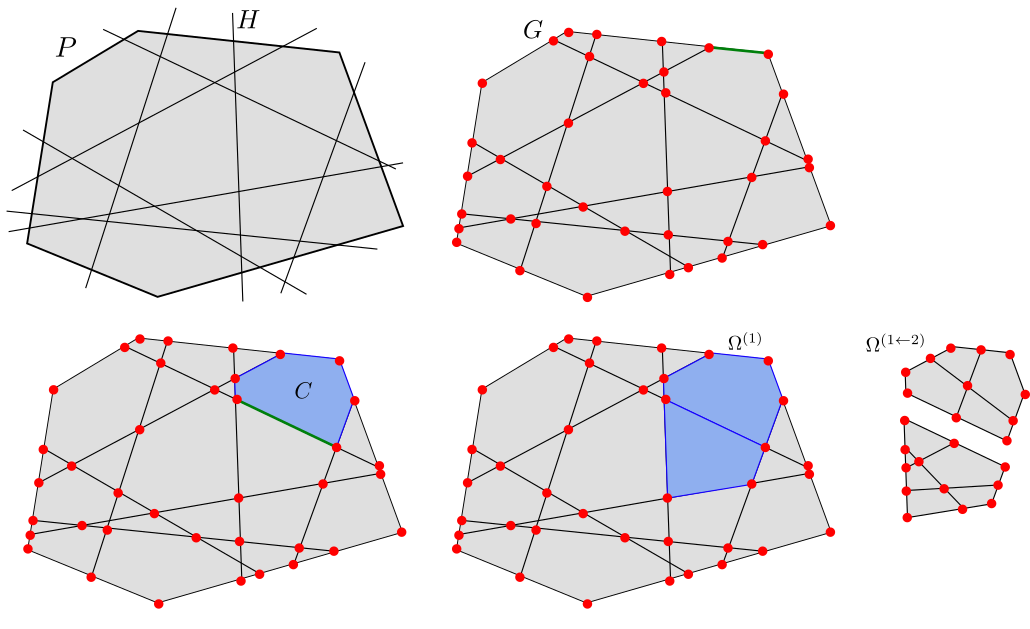
\includegraphics[width=0.8\linewidth]{drawings/splinecam_algorithm.png}
    \caption{The SplineCam visualisation procedure starts by identifying a two-dimensional region of interest $P$ and intersecting it with hyperplanes $H$, \textbf{upper left}. Then a graph $G$ is constructed using the points of intersection as nodes and the hyperplanes and region of interest as edges; an edge is then selected, \textbf{upper right}. A cycle from the selected edge is generated using a breadth first search to identify edges which are then connected in an order; one of the identified edges is then selected, \text{lower left}. With the selected edge, another cycled is formed as before to continue the formation of $\Omega^{(1)}$, \textbf{lower middle}. Once all cycles are identified, the regions are considered individually and intersected with the hyperplanes from the second layer, and the process repeats, \textbf{lower right}.}
    \label{fig:splinecam_algorithm}
\end{figure}

\begin{proposition}\label{prop:complexity_splinecam}
    Given a set of $n$ intersecting hyperplanes and a two-polytope $P$, Algorithm \ref{alg:cycles} has an average case complexity of $O\left(n^2\right)$.
\end{proposition}

\begin{tproof}
    The number of intersections and cycles induces by intersecting a polytope and hyperplanes is on the order less than or equal to $O\left(n^2\right)$. Therefore, the average case complexity of Algorithm \ref{alg:cycles} is also of the order $O\left(n^2\right)$.
\end{tproof}

\section{References}

Chapter \ref{ch:visualisation} from \cite{humayunSplineCamExactVisualization2023}.